\documentclass{scrartcl}
\usepackage[a4paper,left=1in,right=1in,top=1.2in,bottom=1in]{geometry}
\usepackage{siunitx}
\usepackage{graphicx}
\setkomafont{disposition}{\normalfont\bfseries}

%title
\title{Exercise 08:\\Maximum Likelihood Inference}
\subtitle{Theoretical Neuroscience I}
\author{Maria del Cerro \and Johannes G\"atjen \and Lorena Morton}

%use these for structure/overview
\newcommand\Question{%
  \textbf{Question:}%
}
\newcommand\Answer{%
  \textbf{Answer:}%
}

\begin{document}
\maketitle

We are given a function that generates noisy responses of a population of four neurons to a stimulus, as well as a function that calculates the prior probability distribution for stimuli and corresponding responses. First we calculate and analyze the conditional likelihoods for a stimulus $s$ given a response $x$, using the prior probabilities (Figure \ref{cond}). Then we look at three examples of a population response and calculate the most likely stimuli using the conditional likelihoods for the stimuli (Figure \ref{log_ll}). Finally, we analyze how well the population of neurons can decode different stimuli as a whole (Figure \ref{decode}).

\begin{figure}[h]
\centering
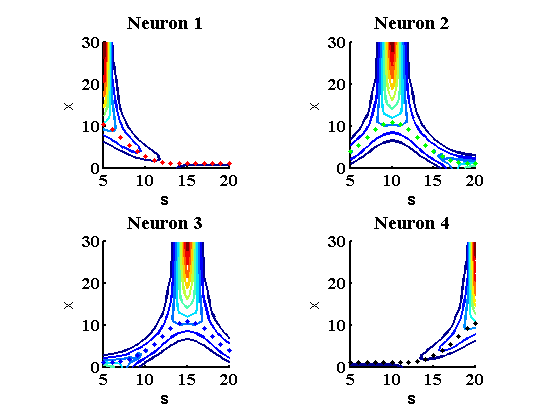
\includegraphics[trim = {1.3cm 0 2cm 0.3cm}, width=0.6\textwidth, clip]{../pics/cond_pdf}
\caption{The contour lines show the conditional likelihood $P_n(s|x)$, i.e. the likelihood for a stimulus $s$, given a response $x$ by neuron $n$. The dots show the expected/average response to a given stimulus. From these graphs, we can identify the preferred stimuli for the four neurons: They are 5, 10, 15 and 20 for neurons 1 through 4 respectively.}
\label{cond}
\end{figure}

\begin{figure}
\centering
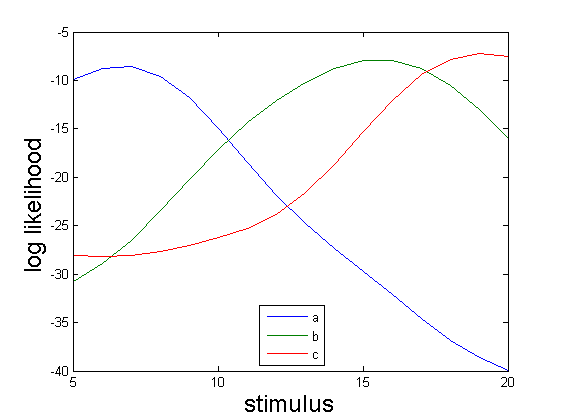
\includegraphics[trim = {0.6cm 0 1.2cm 0.6cm}, width=0.6\textwidth, clip]{../pics/log_ll}
\caption{We are given three population responses $a$, $b$ and $c$. For each response and possible stimulus value, we calculate the log likelihood of that stimulus having occurred when we observe the corresponding response. Selecting the stimulus with the largest log likelihood yields the stimulus that is most likely to have occurred. For responses $a$, $b$ and $c$, these are stimuli 7, 15 and 19 respectively.}
\label{log_ll}
\end{figure}

\begin{figure}
\centering
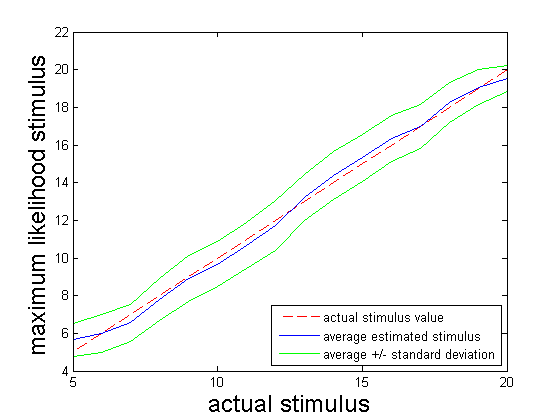
\includegraphics[trim = {0.6cm 0 1.2cm 0.6cm}, width=0.6\textwidth, clip]{../pics/decode}
\caption{For every possible stimulus we compute the average maximum likelihood stimulus $s_\mathrm{ML}$ and the standard deviation of the $s_\mathrm{ML}$. The graph shows the average together with the standard deviation as a function of the true stimulus. Most stimuli are encoded approximately equally well, both in terms of accuracy and precision. The average $s_\mathrm{ML}$ is close to the true stimulus and the standard deviation is almost constant. Only near the edges, for stimuli 5 and 20, the $s_\mathrm{ML}$ is less accurate and the standard deviation is also smaller.}
\label{decode}
\end{figure}
\end{document}